
\documentclass[a4paper]{article}
\usepackage[spanish]{babel}
\usepackage[utf8]{inputenc}
\usepackage{charter}   % tipografia
\usepackage{graphicx}
%\usepackage{makeidx}
\usepackage{paralist} %itemize inline

%\usepackage{float}
%\usepackage{amsmath, amsthm, amssymb}
%\usepackage{amsfonts}
%\usepackage{sectsty}
%\usepackage{charter}
%\usepackage{wrapfig}
\usepackage{listings}
%esto es para formateo del codigo C++
\lstset{
	belowcaptionskip=1\baselineskip,
	basicstyle=\footnotesize,        % the size of the fonts that are used for the code
  	breaklines=true,                 % sets automatic line breaking
  	captionpos=b,                    % sets the caption-position to bottom
  	extendedchars=true,              % lets you use non-ASCII characters; for 8-bits encodings only, does not work with UTF-8
  	keepspaces=true,                 % keeps spaces in text, useful for keeping indentation of code (possibly needs columns=flexible)
  	columns=flexible
  }

%\usepackage{color} % para snipets de codigo coloreados
\usepackage{fancybox}  % para el sbox de los snipets de codigo

\definecolor{litegrey}{gray}{0.94}

% \newenvironment{sidebar}{%
% 	\begin{Sbox}\begin{minipage}{.85\textwidth}}%
% 	{\end{minipage}\end{Sbox}%
% 		\begin{center}\setlength{\fboxsep}{6pt}%
% 		\shadowbox{\TheSbox}\end{center}}
% \newenvironment{warning}{%
% 	\begin{Sbox}\begin{minipage}{.85\textwidth}\sffamily\lite\small\RaggedRight}%
% 	{\end{minipage}\end{Sbox}%
% 		\begin{center}\setlength{\fboxsep}{6pt}%
% 		\colorbox{litegrey}{\TheSbox}\end{center}}

\newenvironment{codesnippet}{%
	\begin{Sbox}\begin{minipage}{\textwidth}\sffamily\small}%
	{\end{minipage}\end{Sbox}%
		\begin{center}%
		\vspace{-0.4cm}\colorbox{litegrey}{\TheSbox}\end{center}\vspace{0.3cm}}



\usepackage{fancyhdr}
\pagestyle{fancy}

%\renewcommand{\chaptermark}[1]{\markboth{#1}{}}
\renewcommand{\sectionmark}[1]{\markright{\thesection\ - #1}}

\fancyhf{}

\fancyhead[LO]{Sección \rightmark} % \thesection\ 
\fancyfoot[LO]{\small{Nombre Apellido, Nombre Apellido, Nombre Apellido}}
\fancyfoot[RO]{\thepage}
\renewcommand{\headrulewidth}{0.5pt}
\renewcommand{\footrulewidth}{0.5pt}
\setlength{\hoffset}{-0.8in}
\setlength{\textwidth}{16cm}
%\setlength{\hoffset}{-1.1cm}
%\setlength{\textwidth}{16cm}
\setlength{\headsep}{0.5cm}
\setlength{\textheight}{25cm}
\setlength{\voffset}{-0.7in}
\setlength{\headwidth}{\textwidth}
\setlength{\headheight}{13.1pt}

\renewcommand{\baselinestretch}{1.1}  % line spacing


% \setcounter{secnumdepth}{2}
\usepackage{underscore}
\usepackage{caratula}
\usepackage{url}


%-------------------para algoritmos
\usepackage[ruled,noend,noline,slide]{algorithm2e}
\usepackage[]{algorithmic}
%-------------------------------------------------
\usepackage{amsmath}


% ******************************************************** %
%              TEMPLATE DE INFORME ORGA2 v0.1              %
% ******************************************************** %
% ******************************************************** %
%                                                          %
% ALGUNOS PAQUETES REQUERIDOS (EN UBUNTU):                 %
% ========================================
%                                                          %
% texlive-latex-base                                       %
% texlive-latex-recommended                                %
% texlive-fonts-recommended                                %
% texlive-latex-extra?                                     %
% texlive-lang-spanish (en ubuntu 13.10)                   %
% ******************************************************** %



\begin{document}


\thispagestyle{empty}
\materia{Algoritmos 3}
\submateria{Segundo Cuatrimestre de 2014}
\titulo{Trabajo Práctico III}
\subtitulo{Algoritmos Sobre Grafos}
\integrante{Ricardo Colombo}{156/08}{ricardogcolombo@gmail.com.com}
\integrante{Federico Suarez}{610/11}{elgeniofederico@gmail.com}
\integrante{Juan Carlos  Giudici}{827/06}{elchudi@gmail.com}
\integrante{Franco Negri}{893/13}{franconegri2004@gmail.com}
\maketitle
\newpage

\thispagestyle{empty}
\vfill

\thispagestyle{empty}
\vspace{3cm}
\tableofcontents
\newpage

%\normalsize

\section{Comparaciones con otros algoritmos conocidos}  
Para este trabajo práctico se nos pide, a partir de un grafo simple $G=(V,E)$ con pesos en las aristas, encontrar la k-particion tal que minimice el peso de las aristas intrapartición.

Para ello primero intentaremos relacionar este problema con otros problemas conocidos, pensaremos varias maneras de abordarlo y emprenderemos la busqueda de algoritmos eficientes para resolverlo.

Como veremos luego, este problema es 'dificil' de resolver, por lo que para instancias grandes, el algoritmo dejará de ser viable, por lo que tambien desarrollaremos distintas heruristicas que resuelvan el problema de manera aproximada. Probaremos con una heuristica golosa, dos heruristicas de busquedas locales y a partir de estos, un GRASP.

\subsection{Entrada y salida}

Todos los algoritmos tomarán como entrada, lo siguiente:

\begin{itemize}
	\item Un entero $\textbf{n}$ $\rightarrow$ Representará el numero de nodos del grafo $G$.

	\item Un entero $\textbf{m}$ $\rightarrow$ Representará la cantidad de aristas del grafo.

	\item Un entero $\textbf{m}$ $\rightarrow$ Representará la cantidad de conjuntos distintos que disponemos para poner los ejes.

	\item $\textbf{m}$ filas donde, para cada fila $i$ consta de $3$ enteros:
	\begin{itemize}
		\item $\textbf{u v w}$ $ \rightarrow $ donde $\textbf{u}$ y $\textbf{v}$ son los nodos adyacentes y $\textbf{w}$ el peso de las aristas entre ellos.
	\end{itemize}
\end{itemize}

La salida, por su parte, constar\'a de una fila con:

\begin{itemize}

	\item $n$ enteros $i_1$ $i_2$ $...$ $i_n$

\end{itemize}

Donde cada $i_k$ representa en que conjunto se encuentra el nodo $k$

\subsection{Ejemplo}

Para ejemplificar el problema a resolver, pensemos en un grafo $G$ con $4$ nodos, $5$ vertices y $2$ particiones.

Supongamos ademas que los nodos estan conectados de la siguiente manera:

\begin{itemize}

	\item $1-2$ con peso $2$
	\item $1-3$ con peso $3$
	\item $1-4$ con peso $3$
	\item $2-4$ con peso $1$
	\item $3-4$ con peso $2$

\end{itemize}

A primera vista podríamos elegir el nodo con mas aristas, el nodo $1$, y ponerlo en una partición obteniendo k-PMP = \{\{($1$)\},\{\}\}. Por otro lado tenderíamos a poner nodos que no esten conectados en otra partición, por ejemplo los nodo $2$ y $3$ ya que estos no los conecta ninguna arista, obteniendo k-PMP = \{\{($1$)\},\{($2$),($3$)\}\}. Ahora en nuestro ejemplo nos queda el nodo $4$ y al tener $k = 2$ lo tenemos que poner en alguna, elegiremos la partición donde minimice el peso total, en este caso es indiferente, dado que agregar el nodo $4$ a la primer partición suma $3$ y a la segunda partición también suma $3$, resultando k-PMP = \{\{($1$),($4$)\},\{($2$),($3$)\}\}. 

De esta forma, mas adelante vamos a ver que un algoritmo goloso que intentase resolver este problema con un esquema similar a lo descripto podria llegar a generar soluciónes tan malas como se quiera.

\subsection{Relación con el problema 3 del Trabajo Práctico 1}

... completar ...

\subsection{Relación con el problema de Colorear un Grafo}

Vamos a relacionar el problema de $k-PMP$ con el problema de coloreo. Supongamos que podemos encontrar un k-coloreo para los vértices del grafo G, entonces podríamos subdividir al conjunto de vértices V en k subgrupos según su color, es decir, en un mismo grupo sólo habrá vertices que compartan color, generando la siguiente partición: k-PMP = \{ $V_1$, ..., $V_k$ \}. 

Por la definición de coloreo, dos vértices de un mismo color no pueden tener aristas entre sí, por lo tanto los grupos que armamos son conjuntos independientes. Esto quiere decir que cada k-partición no tiene aristas intrapartición ya que cada una es un conjunto independiente, luego el peso total de la misma es $0$. Además es un peso mínimo ya que no hay aristas con peso negativo, obteniendo la mejor solución a nuestro problema.

Hasta aquí hemos visto que con un coloreo igual a k se obtiene la solución al problema, pero observemos que los conjuntos de la k-partición resultado no tienen que ser necesariamente no vacíos, lo que nos lleva a pensar que también nos bastaría conseguir un coloreo menor a k para resolver nuestro problema y ahora veremos cómo puede ser esto posible. Dado un k'-coloreo con $k'<k$, por lo dicho anteriormente podemos armarnos k' subgrupos de vértices agrupandolos por color, los cuales serán conjuntos independientes, es decir, no existirán aristas que incidan en dos nodos de un mismo grupo. Sin embargo, ya no me queda ningún vértice para meter en algún grupo y el problema me pide k particiones, por lo que me estarían faltando otras $k-k'$ particiones más que agregar a mi k-partición. Pero si recordamos nuestra observación que decía que las particiones no deben ser necesariamente no vacías, entonces podríamos agregar a nuestra k-partición $k-k'$ particiones de vértices vacías, con lo cual no estaríamos agregando ninguna arista intrapartición. Entonces mis k' particiones iniciales, por lo visto previamente, no tienen ninguna arista intrapartición y los conjuntos vacíos que agregué posteriormente claramente tampoco tienen aristas intrapartición, por lo que he llegado nuevamente a una k-partición de peso $0$, la cual es solución de mi problema y además es óptima.

Por otro lado, dada una solución al problema de k-PMP de peso estrictamente mayor a $0$ para un grafo G determinado, podemos afirmar que no existe un k-coloreo para ese grafo. Si existiera un k-coloreo para dicho grafo, entonces, por lo probado en el anterior párrafo, también existiría una k-PMP de peso $0$ para tal grafo, lo cual es absurdo ya que partimos de una k-PMP de peso estrictamente mayor a $0$.

\clearpage


\section{Algoritmo Exacto}  
\subsection{Introducción}

Dado un grafo simple G = ( V , E ) se quiere buscar la solución con un algoritmo exacto a el problema de la k- partición, para esto se realiza un algoritmo con la técnica de backtracking para obtener la solución exacta del problema.

En los puntos siguientes  se detalla la solución del mismo definiendo la implementación del algoritmo, las podas y  como afectan a la solución en los tiempos.

\subsection{Desarrollo}
Para explicar el desarrollo de este algoritmo iremos mostrando las partes del algoritmo armando el algoritmo final paso a paso, para comenzar el desarrollo es necesario definir previamente cada una de las estructuras que se utilizan en el mismo. Sabemos que el grafo esta representado por un conjunto de vértices, cada uno de los mismos tiene una etiqueta en este caso es un numero desde 1 hasta n  (siendo n la cantidad de vértices del grafo),  a su vez tenemos un conjunto de tuplas que representan los ejes en el grafo cada coordenada tiene un numero del 1 al n representando que vértices conecta el eje, a nuestro grafo lo representamos en una matriz de adyacencias a la que denominamos adyacencias en el grafo, donde en cada posición se tiene 0 si las aristas no están conectadas o el valor del peso del eje en caso que estén conectados.

Una solución será representada en un conjunto de k subconjuntos, donde cada uno de estos subconjuntos contendrá los números de los vértices, todos disjuntos de a pares ( ósea que no tenemos el mismo numero de vértice en dos subconjuntos), y el peso del conjunto será la suma de cada uno de los pesos de los subconjuntos, donde el peso del subconjunto se entienden a la suma de los pesos de las aristas que conecten dos vértices del mismo subconjunto , además definimos que una k partición A es mejor que otra B si el peso total es menor, es decir si A es mejor que B entonces peso(A) < peso(B). Nuestro solFinal en principio va a ser el conjunto donde todos los vértices estén en el primer subconjunto.
La idea fundamental del algoritmo de Backtracking  es que en cada llamado recursivo intentara insertar un vértice a la solución que esta armando, en caso de no tener una mejor solución tratara de insertar ese vértice en otro subconjunto que no haya probado, así hasta haber probado todos los subconjuntos y sin ir mas lejos si se realiza este ejercicio estaremos realizando todas las combinaciones de los vértices en los k subconjuntos.	

De la siguiente manera:
\begin{algorithm}
  \begin{algorithmic}[1]\parskip=1mm
 \caption{ backtracking(solParcial,solFinal,numeroVertice,cantidadSubConjuntos)}
 		\STATE{Si Puedo insertar } 
		\STATE{\quad para cada i desde 1 hasta cantidadSubConjuntos: }
 		\STATE{\quad\quad agrego el numeroVertice al subconjunto i en SolParcial}
 		\STATE{\quad\quad backtracking ( solParcial , solFinal, numeroVertice+1,k,adyacencias)}
		\STATE{\quad\quad saco el elemento que agregue al ultimo conjunto}
		\STATE{Si Puedo insertar }   
		\STATE{devuelvo False}
  \end{algorithmic}
  \end{algorithm}


Ahora de esa manera lo único que estamos haciendo es probar todas las combinaciones , pero no estamos quedándonos con la mejor k - partición para esto debemos definir una función que nos diga cuando una solución es mejor que otra y además debemos saber si ya insertamos todos los vértices.

Para lo cual definimos una función que devuelve un numero indicando 0 si inserte todos los vértices llegando a otra solución, luego tengo que ver si es mejor que la que tengo hasta el momento y 1 si tengo que seguir insertando vértices.
Quedándonos de la siguiente manera:

\begin{algorithm}
  \begin{algorithmic}[1]\parskip=1mm
 \caption{numero check(adyacencias, solParcial,solFinal, numeroVertice,cantidadVertices)}
 		\STATE{SI numeroVertice=cantidadDeVertices }   
 		\STATE{\quad devolver 0}
 		\STATE{SI NO}
		\STATE{\quad devolver 1}
  \end{algorithmic}
  \end{algorithm}
    
\begin{algorithm}
  \begin{algorithmic}[1]\parskip=1mm
 \caption{backtracking(solParcial,solFinal,numeroVertice,cantidadSubConjuntos,adyacencias, cantidadVertices)}
 		\STATE{entero resultadoCheck = check(adyacencias,solParcial,solFinal,numeroVertice,cantidadVertices) }   
 		\STATE{si resultadoCheck = 0 }   
 		\STATE{\quad Remplazo mi solFinal por solParcial}
 		\STATE{Si NO}
		\STATE{\quad para cada i desde 1 hasta cantidadSubConjuntos: }
 		\STATE{\quad\quad agrego el numeroVertice al subconjunto i en SolParcial}
 		\STATE{\quad\quad backtracking ( solParcial , solFinal, numeroVertice+1,k,adyacencias)}
		\STATE{\quad\quad saco el elemento que agregue al ultimo conjunto}
		\STATE{devuelvo False}

  \end{algorithmic}
  \end{algorithm}

Con este algoritmo estaremos probando todas las combinaciones de todos los vértices en los k subconjuntos, en cada paso insertamos un vértice a un subconjunto y llamamos a la recursión con el siguiente vértice. una vez que vuelva de la recursión quitara el vértice del conjunto donde lo ingreso y seguirá el ciclo insertándolo en otro subconjunto y llamando a la recursión de nuevo.

\subsection{Podas}
Para mejorar los tiempos del algoritmo es necesario realizar algún tipo de validación intermedia para no probar casos que no nos van a llevar a una solución optima, por ejemplo cuando estamos insertando vértices a la solución que ya tiene mas peso que nuestra mejor solución o cuando nos quedan una cantidad de vértices es menor estricta a la cantidad de subconjuntos vacíos, estas podas son las que realizamos en nuestro algoritmo agregándolas a la función check al Backtracking de la siguiente manera:

\begin{algorithm}
  \begin{algorithmic}[1]\parskip=1mm
 \caption{numero check(adyacencias, solParcial,solFinal, numeroVertice,cantidadVertices)}
 		\STATE{SI peso(solParcial)$ >$ peso(solFinal) }   
 		\STATE{\quad devolver 2}
		\STATE{SI numeroVertice=cantidadDeVertices }   
 		\STATE{\quad devolver 0}
 		\STATE{Si cantidadDeCajasVacias(solParcial)$ >$ cantidadVertices }   
 		\STATE{\quad devolver 2}
		\STATE{devolver 1}
  \end{algorithmic}
  \end{algorithm}
La funcion cantidadDeCajasVacias se fija si algun conjunto no tiene  
 
 \begin{algorithm}
 \begin{algorithmic}[1]\parskip=1mm
 \caption{backtracking(solParcial,solFinal,numeroVertice,cantidadSubConjuntos,adyacencias, cantidadVertices)}
 		\STATE{entero resultadoCheck = check(adyacencias,solParcial,solFinal,numeroVertice,cantidadVertices) }   
 		\STATE{si resultadoCheck = 0 }   
 		\STATE{\quad Remplazo mi solFinal por solParcial}
		\STATE{si resultadoCheck = 2 }   
 		\STATE{\quad devuelvo false porque mi solParcial es peor que mi solFinal o tengo mas cajas vacías que vertices para poner	l}
 		\STATE{Si NO}
		\STATE{\quad para cada i desde 1 hasta cantidadSubConjuntos: }
 		\STATE{\quad\quad agrego el numeroVertice al subconjunto i en SolParcial}
 		\STATE{\quad\quad backtracking ( solParcial , solFinal, numeroVertice+1,k,adyacencias)}
		\STATE{\quad\quad saco el elemento que agregue al ultimo conjunto}
		\STATE{devuelvo False}
  \end{algorithmic}
  \end{algorithm}

De esta manera el algoritmo va a realizar las podas en las llamadas recursivas intermedias antes de insertar todos los vértices descartando casos que no son útiles para llegar  a una solución optima en menor tiempo.

Para improvisar una mejora en la poda al comparar los pesos de nuestras soluciones parcial y final, lo que realizamos es generar otra solución final asignando cada uno de los vértices de manera creciente a cada uno de las k subconjuntos diferentes y si esta otra solución es mejor a la solución que tiene todos los nodos en un solo conjunto la tomamos como solución final para nuestras comparaciones.
De esta manera podrían tomarse otro tipo de soluciones para luego obtener la solución final de menor peso y podar mas ramas del Backtracking.	

\subsection{Complejidad}
Dado que el algoritmo exacto sin las podas prueba todas las soluciones del problema esto hace que sea poco eficiente en terminos de tiempo a comparacion de las heuristicas que iremos viendo a lo largo del informe. Pero conociendo las soluciones que se van a ir armando pueden definirse podas para evitar seguir resolviendo ramas de la solucion que no me van a llevar a una solucion optima o a una solucion que no es mejor que la que ya forme hasta cierto punto.
Dado el algoritmo exacto mostraremos las complejidades de las diferentes partes del mismo para obtener cual seria la complejidad final.

\begin{algorithm}
  \begin{algorithmic}[1]\parskip=1mm
 \caption{numero check(adyacencias, solParcial,solFinal, numeroVertice,cantidadVertices)}
 		\STATE{SI peso(solParcial) $>$ peso(solFinal)  \tOde{1}}   
 		\STATE{\quad devolver 2}
		\STATE{SI numeroVertice=cantidadDeVertices \tOde{1} }   
 		\STATE{\quad devolver 0}
 		\STATE{Si cantidadDeCajasVacias(solParcial) $>$ cantidadVertices \tOde{k}}   
 		\STATE{\quad devolver 2}
		\STATE{devolver 1}
  \end{algorithmic}
  \end{algorithm}

Para la funcion check la complejidad final sera \Ode{1} + \Ode{1}+ \Ode{k} dando como complejidad total \tOde{k}.

\begin{algorithm}
 \begin{algorithmic}[1]\parskip=1mm
 \caption{backtracking(solParcial,solFinal,numeroVertice,cantidadSubConjuntos,adyacencias, cantidadVertices)}
 		\STATE{entero resultadoCheck = check(adyacencias,solParcial,solFinal,numeroVertice,cantidadVertices)\tOde{k} }   
 		\STATE{si resultadoCheck = 0 \tOde{1}}   
 		\STATE{\quad Remplazo mi solFinal por solParcial \tOde{k}}
		\STATE{si resultadoCheck = 2 \tOde{1}}   
 		\STATE{\quad devuelvo false porque mi solParcial es peor que mi solFinal o tengo mas cajas vacías que vertices para poner \tOde{1}}
 		\STATE{Si NO}
		\STATE{\quad para cada i desde 1 hasta cantidadSubConjuntos: }
 		\STATE{\quad\quad agrego el numeroVertice al subconjunto i en SolParcial}
 		\STATE{\quad\quad backtracking ( solParcial , solFinal, numeroVertice+1,k,adyacencias)}
		\STATE{\quad\quad saco el elemento que agregue al ultimo conjunto}
		\STATE{devuelvo False}
  \end{algorithmic}
  \end{algorithm}

El ciclo de las lineas 7-10 se ejecuta k veces en cada llamado iterativo, cada ves que se llama a la funcion backtracking es por un vertice diferente. 
Para el primer nodo tenemos k conjuntos para probar, luego con el segundo vertice tenemos para cada uno de esos conjuntos donde coloque el primer nodo k alterativas de conjuntos para probar quedandonos $k^2$ combinaciones para esos dos vertices,
para cada una de esas $k^2$ combinaciones tenemos k conjuntos quedando $k^3$ combinaciones, asi seguira en las llamadas recursivas por todos los vertices. Con lo cual con el vertice n tendremos $k^n$ combinaciones para este vertice.

Por lo tanto la complejidad total del algortimo es del orden de \Ode{$k^n$} siendo k la cantidad de subconjuntos y n la cantidad de vertices del grafo.

\subsection{Experimentacion}
Para el analisis de este algoritmo se generaron 30 instancias de manera random de grafos completos con vertices entre 1 y 20 elegidos de manera aleatoria mediante un script en python con la funcion randint.
Luego para esas instancias se corrio el algoritmo asignando 5, 10 y 15 subconjuntos para ver como se comportaba el algoritmo, obteniendose como resultado lo siguiente:\\
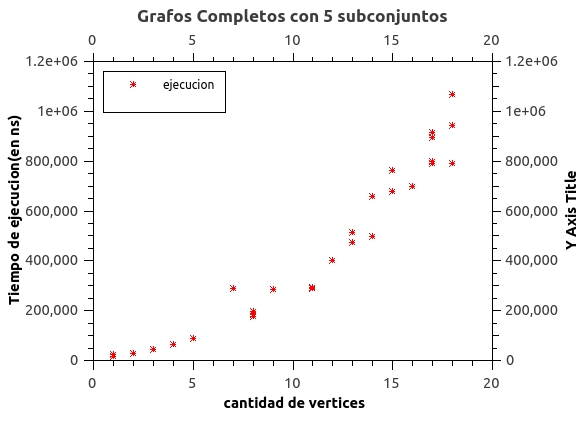
\includegraphics[scale=0.5]{Ej2/k5.jpg}
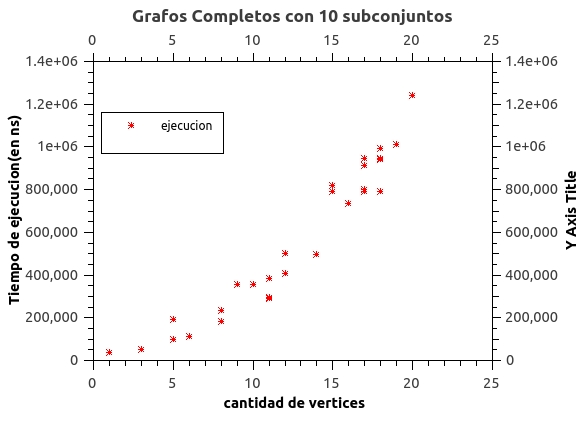
\includegraphics[scale=0.5]{Ej2/k10.jpg}\\
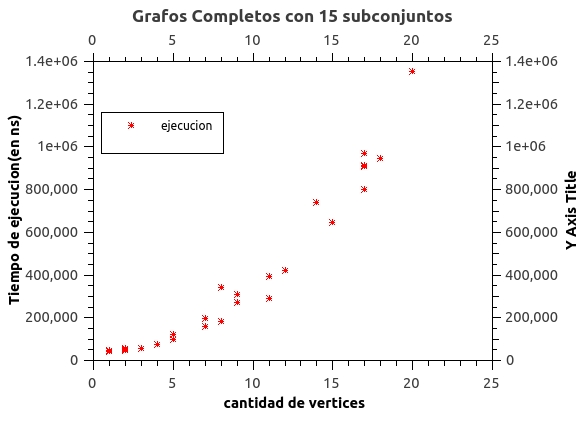
\includegraphics[scale=0.5]{Ej2/k15.jpg}\\

Se puede ver como la curva se hace mas pronunciada al cambiar la cantidad de subconjuntos, con esto se ve que al cambiar el k la complejidad va aumentando de manera exponencial.

Por otro lado realizamos un analisis sobre las podas, para esto primero generamos 30 instancias de grafos para ver como se comportaba el algoritmo con grafos sin aristas, obteniendo el siguiente resultado:\\
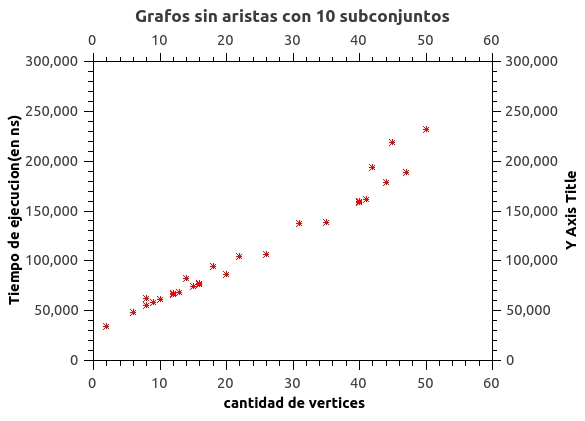
\includegraphics[scale=0.5]{Ej2/sinAristas.jpg}\\
Como puede verse el grafico los tiempos de ejecucion son similares a una lineal, esto se debe a que como la solucion inicial tiene peso 0 ya que no tiene aristas, en cada llamado recursivo se devuelve false porque no se obtiene nada mejor en cuestion de peso del conjunto.
Por otro lado como mencionamos en el desarrollo del algoritmo se agrego una genacion de una solucion inicial alternativa a poner todos los vertices en un solo subconjunto, por lo que realizamos una experimentacion para ver como afectaba la no presencia de esta solucion alternativa, corrimos las mismas instancias de grafos para 15 subconjuntos que corrimos en los priemros test donde se encontraba esta solucion alternativa y obtuvimos lo siguiente:\\
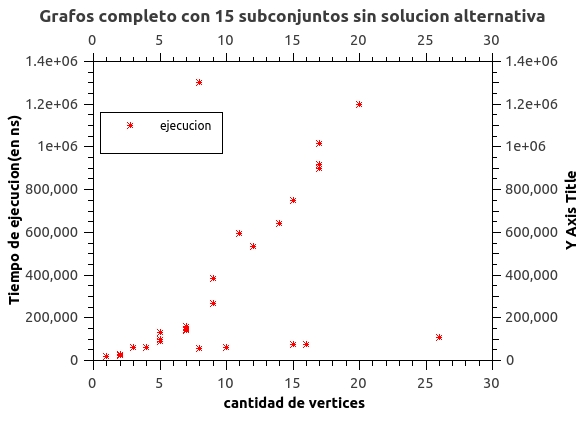
\includegraphics[scale=0.5]{Ej2/sinAlternativa.jpg}\\

Como puede observarse los tiempos empeoran ya que la primera solucion a nuestro problema es el grafo con todos las aristas y esto puede no podar muchas ramas del backtracking que con la solucion alternativa si se estan podando. Concluyedo que podrian mejorar los tiempos si estamos eligiendo una buena solucion inicial.



\clearpage


\section{Heuristica Golosa Constructiva} 
\subsection{Idea general}

Un primer intento para conseguir una solución a este problema es utilizando un algoritmo goloso. La idea del mismo es sencilla, numeramos los nodos de $1$ a $n$, y luego tomando de a uno los agregamos a alguno de los conjuntos de $1$ a $k$ intentando que sume a la solución el menor peso posible.

Mas formalizado el algoritmo quedará de la siguiente manera:


\begin{algorithm}
  \begin{algorithmic}[1]\parskip=1mm
 \caption{ Goloso()}
 		\STATE{Numero los vertices de $1$ a $n$} 
		\STATE{Creo una cantidad $k$ de conjuntos donde iré guardando vertices}
 		\STATE{Para cada nodo $i$ de $1$ a $n$: }
		\STATE{\quad Para cada conjunto}
			\STATE{\quad\quad Sumo todos los pesos de las aristas de ($i$,$j$) con $j$ los vertices que estan en el conjunto}
 		\STATE{\quad Agrego la el vertice $i$ para el cual la suma dio menor}
		\STATE{Imprimo por salida estandar la respuesta}
  \end{algorithmic}
  \end{algorithm}


Claramente este algoritmo no devuelve la solución exacta, y como se verá mas adelante, la solución que devuelve puede estar tan lejos como se quiera de la optima, lo que lo hace un algoritmo no muy bueno.

El analisis de complegidad es sencillo, se itera por cada vertice sobre cada conjunto. Dado que cada nodo solo estará en un conjunto, entre todos los conjuntos a lo sumo tendrán $n$ nodos, lo que hace que se deba iterar $n$ veces a lo sumo sobre $n$ nodos, luego la complegidad será $O(n^2)$, por lo que, al menos en lo que respecta a tiempos, es ampliamente superior que el algoritmo exacto.

Por lo tanto, dada la baja complegidad de este algoritmo, podría utilizarse como una cota superior, si bien algo grosera, para la solución.

\subsection{Problemas del Algoritmo Goloso}

Como ya adelantamos, la solución para este algoritmo no siempre da una solución exacta, y puede ser tan mala como se quiera. Esto surge principalmente de darle un orden a los nodos, como mostraremos en el siguiente ejemplo.

Supongamos que tenemos un grafo como el que se muestra en la figura y $K = 2$

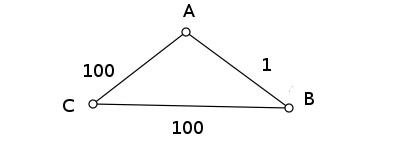
\includegraphics[scale=0.5]{Ej3/grafo.png}

Es claro que la mejor solución posible es poner en uno de los conjuntos a $A$ y $B$ y en el otro a $C$, así la suma intrapartición es $1$.

Sin embargo, supongamos que nuestro algoritmo goloso toma como primer nodo al nodo $A$, dado que no hay otros nodos, lo agrega en cualquiera de los dos conjuntos y se obtiene peso $0$. Ahora supongamos que el algoritmo toma el nodo $B$, si lo pone en el mismo conjunto que el nodo $A$ obtiene peso $1$, si lo pone en el otro conjunto obtiene peso $0$, asi que lo pone en el otro conjunto. Pero ahora falta agregar el nodo $C$, y agregandolo en cualquiera de los dos conjuntos se obtiene peso $100$. Asi que la solución para k-PMP que encontrará el algoritmo goloso será $100$.
De ahí se desprende que cambiando ambos pesos $100$ por cualquier valor puede obtenerse una solución tan mala como uno quiera.

Sin embargo, puede observarse otra cosa de este algoritmo, si se hubiese tomado el nodo $C$ como primer nodo o como segundo nodo, se hubiera llegado a la solución optima. De aquí surge la idea de que si se eligieran diferentes ordenes para los nodos y se corriera el algoritmo para cada uno de estos ordenes, podría obtenerse diferentes cotas, y con un poco de suerte en alguna de ellas no sucederá este caso que acabamos de ver.

Esta idea la utilizaremos mas adelante para el GRASP, correremos con distintos ordenes de nodos el algoritmo goloso de manera tal de obtener en cada una de estas iteraciones una respuesta diferente y posiblemente mejor que la anterior.

\subsection{Testing}

En esta sección, realizaremos diferentes experimentos para comprobar que el algoritmo escala de acuerdo a la complegidad teorica, asi como tambien, veremos que tan buenos resultados obtenemos en la practica para este algoritmo.

Primero se corre el algoritmo con instancias de 25 a 200 nodos y se grafican los tiempos obtenidos:


=== TIEMPOS ===

Dividiendo por una función $f(i) = i^2$ obtenemos que una linea constante, por lo que podemos comprobar asi de manera empirica, que el reslutado obtenido es efectivamente cuadratico.

Ahora tomaremos grafos completos de $23$ nodos (El backtrack es el factor limitante, de tomar mas nodos empieza a tardar un tiempo excesivo), y compararemos los resultados dados tanto por la heuristica golosa como por el backtrack. Cabe notar que las aristas de los grafos serán elegidas al azar entre un numero del 1 al 100 para no tomar casos demasiado particulares que favorezcan a uno u otro algoritmo.

Tomando el promedio, las respuestas que se obtuvieron son las siguientes:

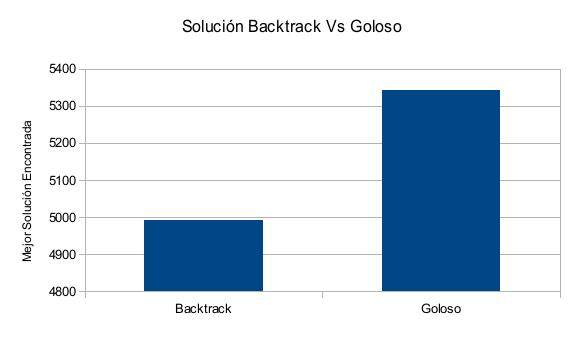
\includegraphics[scale=0.5]{Ej3/Soluciones.jpg}

Como puede verse el algoritmo goloso, en promedio, da soluciónes significativamente peores que la respuesta exacta.

De las anteriores 100 muestras tambien se calculo el tiempo que se tardó en obtener las respuestas, nuevamente promediando se obtiene:

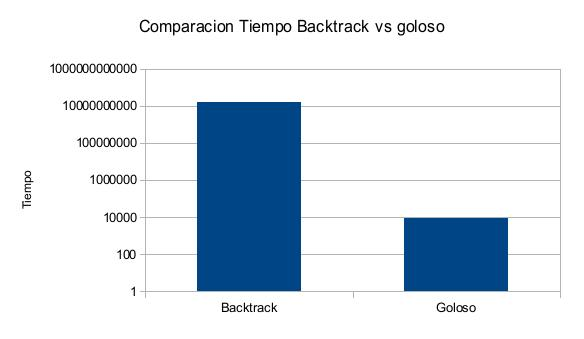
\includegraphics[scale=0.5]{Ej3/tiempos.jpg}

Donde se ve que el algoritmo goloso es $6$ ordenes de magnitud mas rapido que el backtrack, incluso para una instancia modesta de $23$ nodos.


\clearpage

\section{Heuristica de Busqueda Local} 
\section{Introducci\'on}

En esta sección se implementarán heurísticas de búsqueda local para tratar de resolver el problema de $k-PMP$, intentando con diferentes métodos para alcanzar una solución y diferentes vecindades.

Para ello, partiendo de una solución generada al azar, se intentará a través de sucesivas iteraciones analizar cierta vecindad para intentar mejorar la solución existente y aproximarse más a una 'buena' solución en un tiempo aceptable. 

Por lo tanto debemos tener en cuenta de no hacer las vecindades ni muy grandes, ya que esto puede llevar a una pérdida de performance, ni muy pequeñas, ya que esto puede llevar a que el algoritmo explore sólo una pequeña cantidad de soluciones y devuelva una solución muy alejada del óptimo.

Como primera idea para una vecindad tomaremos cada nodo del grafo, vemos cuánto peso agrega en la suma intraconjunto en que se encuentra, lo quitaremos de este conjunto e intentamos meterlo en todos los demás, viendo si en alguno logra minimizar esta suma. En caso afirmativo, lo sacamos de su antiguo conjunto y lo ponemos en el nuevo. Realizamos esto hasta que deja de ser posible mejorar la solución y en este punto la devolvemos.


Otra vecindad que plantearemos será buscar el nodo que más peso está generando en la suma intrapartición, quitarlo de la partición donde se encuentra y agregarlo a alguna otra.

Finalmente se implementará una tercera busqueda local que quite dos nodos que están en una misma partición e intente buscar alguna otra donde los mismos sumen un menor peso intrapartición.

Los algoritmos escritos de manera formal serán así:

\begin{algorithm}
  	\begin{algorithmic}[1]\parskip=1mm
		 \caption{ Busqueda1(SoluciónInicial) }
		 	\STATE{Guardo SoluciónInicial en SolucionPrevia}
	 		\STATE{Mientras en el paso anterior se haya mejorado SolucionPrevia} 
				\STATE{\quad Para todo nodo $i$ de $1$ a $n$ del grafo ~~~~ $\mathcal{O}(n)$}
		 		\STATE{\quad Miro que peso agrega el nodo $i$ en el conjunto asignado por SolucionPrevia  $\mathcal{O}(n)$}
		 		\STATE{\quad Miro que peso agrega el nodo $i$ quitandolo del conjunto asignado y poniendolo en los demas $\mathcal{O}(n)$}
				\STATE{\quad \quad Si algun conjunto $M$ obtengo un peso menor, modifico SolucionPrevia $\mathcal{O}(n^2)$}
				\STATE{\quad \quad Asigno $i$ al conjunto $M$ $\mathcal{O}(1)$}   
				\STATE{\quad \quad Itero}
	\end{algorithmic}
\end{algorithm}

En el paso "Miro qué peso agrega el nodo $i$ quitándolo del conjunto asignado y poniéndolo en los demás", que dado que todo nodo puede estar sólo en un conjunto, iterando sobre todos los elementos de los conjuntos, al menos voy a iterar n veces, de ahí la complejidad $\mathcal{O}(n)$.

Dada nuestra implementación de conjunto con listas simplemente enlazadas, encontrar un elemento y borrarlo cuesta $\mathcal{O}(n^2)$ por esta razón modificar solución previa tendrá esta complejidad. Utilizando listas doblemente enlazadas esto se hubiera podido reducir a $\mathcal{O}(n)$ pero por falta de tiempo no se implementó.

\begin{algorithm}
  	\begin{algorithmic}[1]\parskip=1mm
		 \caption{ Busqueda2(SoluciónInicial) }
			\STATE{Guardo SoluciónInicial en SolucionPrevia}
	 		\STATE{Mientras en el paso anterior se haya mejorado SolucionPrevia}
			\STATE{Asigno $j = 1$}
				\STATE{\quad Tomo el j-esimo nodo mas pesado de la SolucionPrevia, al que llamo $i$ $\mathcal{O}(1)$}
		 		\STATE{\quad Miro que peso agrega el nodo $i$ en el conjunto asignado por SolucionPrevia $\mathcal{O}(n)$}
		 		\STATE{\quad Miro que peso agrega el nodo $i$ quitandolo del conjunto asignado y poniendolo en los demas $\mathcal{O}(n)$}
				\STATE{\quad \quad Si En algun conjunto $M$ obtengo un peso menor}   
				\STATE{\quad \quad \quad modifico SolucionPrevia y asigno $i$ al conjunto $M$ $\mathcal{O}(n^2)$}
				\STATE{\quad \quad \quad Itero}
				\STATE{\quad \quad Si no, sumo $1$ a $j$}
				\STATE{\quad \quad Si $j == n$}
				\STATE{\quad \quad \quad Devuelvo SolucionPrevia}
				\STATE{\quad \quad Si no}
				\STATE{\quad \quad \quad Itero}
	\end{algorithmic}
\end{algorithm}

\begin{algorithm}
  	\begin{algorithmic}[1]\parskip=1mm
		 \caption{ Busqueda3(SoluciónInicial) }
		 	\STATE{Guardo SoluciónInicial en SolucionPrevia}
	 		\STATE{Mientras en el paso anterior se haya mejorado SolucionPrevia} 
				\STATE{\quad Para todo nodo $i$ de $1$ a $n$ del grafo $\mathcal{O}(n)$}
				\STATE{\quad\quad Tomo otro nodo $k$ del mismo conjunto de $i$ $\mathcal{O}(1)$}
		 		\STATE{\quad\quad Miro que peso agrega el nodo $i$ y $k$ en el conjunto asignado por SolucionPrevia $\mathcal{O}(n)$}
		 		\STATE{\quad\quad Miro que peso agrega el nodo $i$ y $k$ quitandolo del conjunto asignado y poniendolo en los demas $\mathcal{O}(n)$}
				\STATE{\quad\quad \quad Si algun conjunto $M$ obtengo un peso menor, modifico SolucionPrevia $\mathcal{O}(n^2)$}
				\STATE{\quad\quad \quad Asigno $i$ y $k$ al conjunto $M$ $\mathcal{O}(1)$}   
				\STATE{\quad\quad \quad Itero}
	\end{algorithmic}
\end{algorithm}

\newpage

\section{Análisis de Complejidades}

Aquí analizaremos las complejidades de los diferentes algoritmos. Para cada uno de ellos elegimos una implementación con matriz de adyacencias para modelar el peso de las aristas y un vector de longitud variable para implementar los diferentes conjuntos.

Para el primero, cada paso de búsqueda local tendrá una complejidad de peor caso de $O(n(n + n + n^2))$. Ahora si $k$ es mayor a $n$ quiere decir que hay más subconjuntos disponibles que nodos, lo que llevaría a una solución trivial donde cada nodo va en un subconjunto diferente y la solución para $k-PMP$ sería 0.
Luego podemos acotar a $k$ por $n$ con lo que se obtendría una complejidad igual a $O(n^3)$

Para el segundo algoritmo, por cada iteración del algoritmo la complejidad será $O(n^2)$ para calcular el nodo con mayor peso del grafo. $O(n)$ para determinar si existe una mejor partición donde este nodo pueda estar y, en el caso de que exista, $O(n^2)$ para quitarlo de la partición anterior y agregarlo a la nueva. Luego, nuevamente acotando $k$ por $n$, se obtiene una complejidad para cada paso de la iteración de $O(n^2)$.

El tercer algoritmo es simplemente el primer algoritmo pero esta vez para cada nodo además tomo un vecino, y realizo el mismo procedimiento que antes, esto para cada vecino, suponiendo que en el peor caso, para un nodo todos los otros nodos esten en el mismo conjunto, se tendrá que realizar el procedimiento de antes la misma cantidad de veces solo que ahora para dos nodos distintos, luego la complejidad continúa siendo $O(n^2 (n + n k + n^2))$. Acotando nuevamente $k$, obtenemos que el algoritmo es: $O(n^3)$

\section{Testing}

En esta sección comprobaremos de manera empírica las complejidades antes calculadas y luego una comparación entre las tres diferentes heurísticas.

Para ello, al igual que para el algoritmo goloso, tomamos grafos completos con 25 a 100 nodos, y comparamos los diferentes tiempos obtenidos:

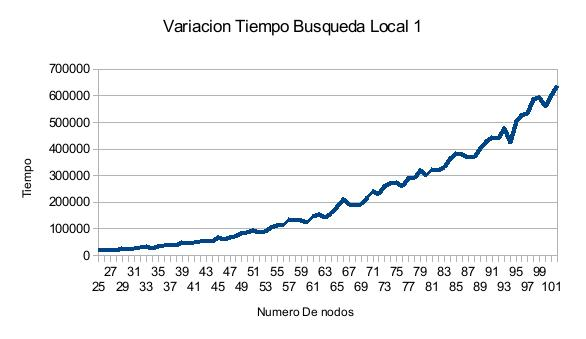
\includegraphics[scale=0.5]{Ej4/tiempo1.jpg}

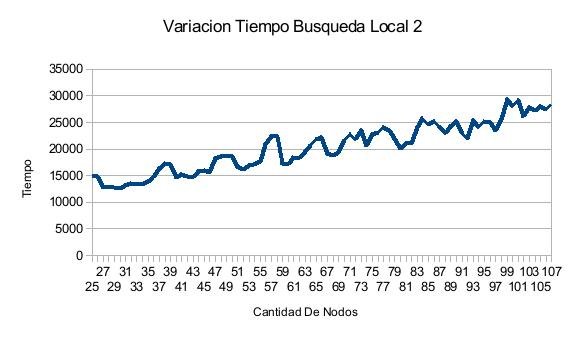
\includegraphics[scale=0.5]{Ej4/tiempo2.jpg}

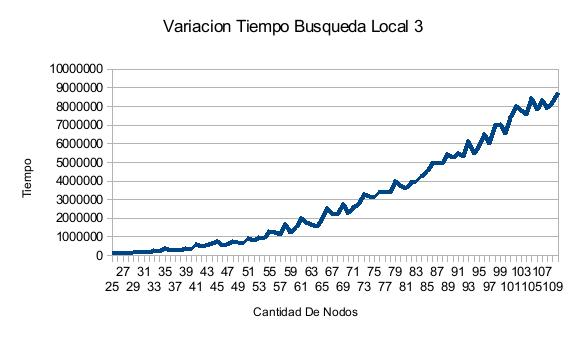
\includegraphics[scale=0.5]{Ej4/tiempo3.jpg}

Puede verse que si bien existe cierto ruido en la toma de muestras, causado muy posiblemente por el hecho de que para cada grafo, el número de veces que es posible continuar mejorando la solución sea variable y poco controlable. Existe una tendencia muy marcada en los tres algoritmos.

Para poner más en evidencia esto, dividiremos por las complejidades teóricas para así hacer más evidente este patrón:

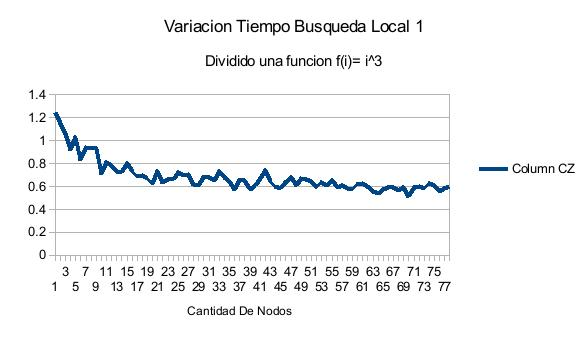
\includegraphics[scale=0.5]{Ej4/tiempo1div.jpg}

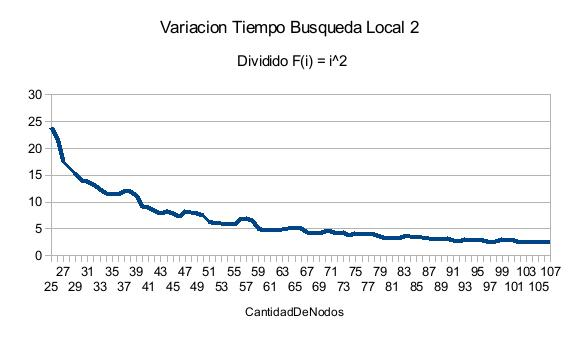
\includegraphics[scale=0.5]{Ej4/tiempo2div.jpg}

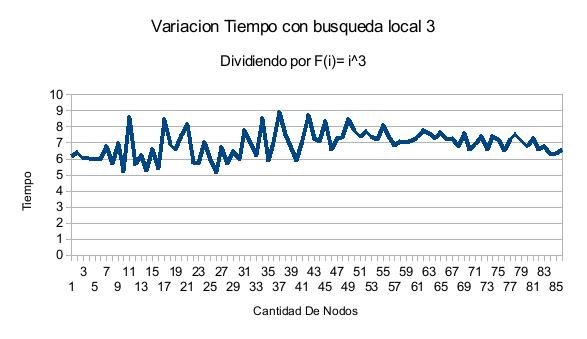
\includegraphics[scale=0.5]{Ej4/tiempo3div.jpg}

Como puede verse, en los tres casos las heurísticas están acotadas por las complejidades calculadas en el apartado anterior.

Veamos como se comportan las busquedas locales contra el algoritmo exactos para $K_23$ con peso en las aristas entre $1$ a $100$ elegidos de forma uniforme, tomaremos 100 muestras y compararemos los resultados contra el algoritmo de backtracking.

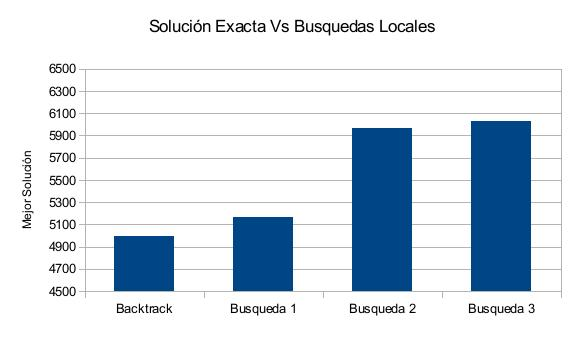
\includegraphics[scale=0.5]{Ej4/solucionestodos.jpg}

Puede verse que el que mejor aproxima a las soluciones reales es la primera búsqueda local. Y no solo eso, de los 100 casos tomados, la búsqueda local 1 logra encontrar la solución exacta a 13 de las instancias! mientras que las otras dos heurísticas en ninguno de los casos logran encontrar la solución exacta.

Además, para estas instancias se realiza a modo comparativo un promedio de los tiempos que tardan en encontrar la solución, esto es lo que se obtiene:

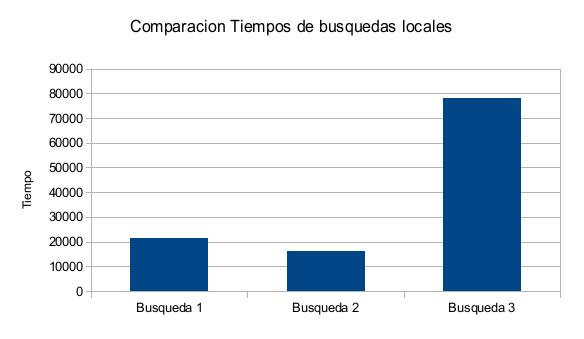
\includegraphics[scale=0.5]{Ej4/tiempotodos.jpg}

Por lo que en primera instancia, el algoritmo de búsqueda local 1 es bastantemente superior en todo sentido a los otros dos, ya que encuentra soluciones exactas y obtiene tiempos empíricos mucho mejores que los otros dos algoritmos.


\clearpage


\section{GRASP} 
\section{Idea}


Para la metaheurística de GRASP, tomaremos el algoritmo goloso previamente implementado y lo combinaremos con las diferentes búsquedas locales también previamente implementadas.

La idea es la siguiente, para cada paso del algoritmo, corremos una versión modificada del goloso de manera tal de permitir cierta aleatoriedad en los resultados. El algoritmo goloso será modificado de la siguiente manera:

\begin{algorithm}
  \begin{algorithmic}[1]\parskip=1mm
 \caption{ Goloso()}
 		\STATE{Numero los vértices de $1$ a $n$} 
		\STATE{Creo una cantidad $k$ de conjuntos donde iré guardando vértices}
 		\STATE{Para cada nodo $i$ de $1$ a $n$: }
		\STATE{\quad Para cada conjunto}
			\STATE{\quad\quad Sumo todos los pesos de las aristas de ($i$,$j$) con $j$ los vértices que están en el conjunto}
 		\STATE{\quad De los mejores $x$ resultados, tomo uno al azar y pongo a $i$ en ese conjunto}
		\STATE{Devuelvo la respuesta}
\end{algorithmic}
\end{algorithm} 

Notar que si $x=1$ entonces estamos obteniendo el mismo algoritmo goloso que en el apartado anterior. En cambio, si tomo $x = k$ (esto es, tomo los $k$ mejores resultados, o sea todos), estaría generando una solución completamente aleatoria. Cualquier solución en medio tomará una solución golosa, pero con cierto grado de aleatoriedad.

Luego a la solución obtenida por el algoritmo goloso modificado se le aplicarán una de las búsquedas locales implementadas en un intento de acercar aún mas la respuesta al óptimo.

Como criterio de corte se correrá el goloso aleatorizado y la busqueda local hasta que luego de que un número $x$, a determinar, de intentos no haya sido posible mejorar la solución. En este punto se entrega la mejor respuesta obtenida hasta el momento.

Dado que tenemos tres busquedas locales, se decide desarrollar tres GRASPs diferentes. Uno con cada una de las busquedas locales. A continuación se formaliza de manera más precisa los algoritmos de cada una:

\begin{algorithm}
  	\begin{algorithmic}[1]\parskip=1mm
		 \caption{ GRASP 1(SoluciónInicial) }
		 \STATE{while(true)}
		 	\STATE{\quad Corro el Algoritmo Goloso modificado}
		 	\STATE{\quad Utilizo búsqueda local 1 para mejorar la solución obtenida previamente}
		 	\STATE{\quad Si conseguí una mejor solución que antes, la guardo}
		 	\STATE{\quad Si tras $z$ iteraciones no se pudo conseguir una mejor solución}
		 	\STATE{\quad\quad Devuelvo la solución}
	\end{algorithmic}
\end{algorithm}

\begin{algorithm}
  	\begin{algorithmic}[1]\parskip=1mm
		 \caption{ GRASP 2(SoluciónInicial) }
		 \STATE{while(true)}
		 	\STATE{\quad Corro el Algoritmo Goloso modificado}
		 	\STATE{\quad Utilizo búsqueda local 2 para mejorar la solución obtenida previamente}
		 	\STATE{\quad Si conseguí una mejor solución que antes, la guardo}
		 	\STATE{\quad Si tras $z$ iteraciones no se pudo conseguir una mejor solución}
		 	\STATE{\quad\quad Devuelvo la solución}
	\end{algorithmic}
\end{algorithm}

\begin{algorithm}
  	\begin{algorithmic}[1]\parskip=1mm
		 \caption{ GRASP 3(SoluciónInicial) }
		 \STATE{while(true)}
		 	\STATE{\quad Corro el Algoritmo Goloso modificado}
		 	\STATE{\quad Utilizo búsqueda local 3 para mejorar la solución obtenida previamente}
		 	\STATE{\quad Si conseguí una mejor solución que antes, la guardo}
		 	\STATE{\quad Si tras $z$ iteraciones no se pudo conseguir una mejor solución}
		 	\STATE{\quad\quad Devuelvo la solución}
	\end{algorithmic}
\end{algorithm}

En estos tres casos $z$ será un numero entero entre $1$ e infinito.

En el siguiente apartado de experimentación se intentarán calibrar tanto el parámetro $x$ como el parámetro $z$ para así obtener los mejores resultados posibles con estas metaheurísticas, tratando siempre de equilibrar performance y exactitud de los resultados.

\section{Experimentación}

Para cada uno de los algoritmos seteamos ambos parametros $x$ y $z$ de manera arbitraria para obtener resultados más o menos adecuados.

Luego para aproximar más estos resultados comenzamos a variar $x$ dejando fijo $z$ y viendo cuales son los cambios en la performance de cada uno de los GRASPs.

Para eso tomamos un grafo completo de $500$ nodos tal que las aristas tienen pesos enteros aleatorios entre $1$ y $100$. Corremos el algoritmo con $x=1$, lo que equivale a una solución inicial obtenida por el algoritmo goloso determinístico, $x=k$ una solución inicial completamente aleatoria, y luego soluciones intermedias para $x = \lfloor0.25 k\rfloor$, $x = \lfloor0.50 k\rfloor$ y $x = \lfloor0.75 k\rfloor$.

Dado que la solución depende fuertemente de $k$ para el grafo antes mencionado, le variaremos el $k$ para tres instancias diferentes con $k = 50$, $k = 200$ y $k = 400$.

Luego los resultados obtenidos para el grafo con $500$ nodos y $k = 50$ son los siguientes:

\includegraphics[scale=0.5]{Ej5/comparacionEntreGrasp50.jpg}

Hasta aquí los resultados parecerían indicar que tomando $x = 1$ pequeño se obtienen resultados muy superiores a los demas casos, tanto en los tiempos obtenidos, como en los conjuntos encontrados.

Se procede a realizar la experimentación para el mismo grafo de $500$ nodos, pero ahora con $k = 200$:

\includegraphics[scale=0.5]{Ej5/comparacionEntreGrasp200.jpg}

Nuevamente podemos observar que para $x = 1$ se obtienen los mejores resultados tanto en performance como en tiempo.

Ahora realizando la experimentación con $k = 400$, se obtiene:

\includegraphics[scale=0.5]{Ej5/comparacionEntreGrasp400.jpg}

De esta manera determinamos que los mejores resultados para este testeo se obtienen con un $x$ fijo igual a $1$. Para ajustar mejor el valor de $x$, ahora tomamos otro grafo de $500$ nodos, y variamos nuevamente el $x$ para valores proximos a $1$. Nuevamente variamos tambien el $k$ para ver como se ven afectados los resultados.





\clearpage

\section{GRASP} 
\section{Experimentacion Final}
Ahora, para concluir este trabajo, tomamos todos los algoritmos antes vistos y realizamos una experimentacion conjunta entre todos para mostrar como se comparan entre si.

La primera de las experimentaciones se realizará con grafos completos de 23 vertices con atistas elegidas al azar del 1 al 100. Sobre cada una de estas instancias se correrán todos los algoritmos antes descriptos, se tomarán cual es la mejor solucion encontrada por el mismo y cuanto tarda en encontrarla y en base a los resultados obtenidos se graficarán en una tabla comparativa donde puedan verse los resultados.

De esta experimentación, se obitiene que:

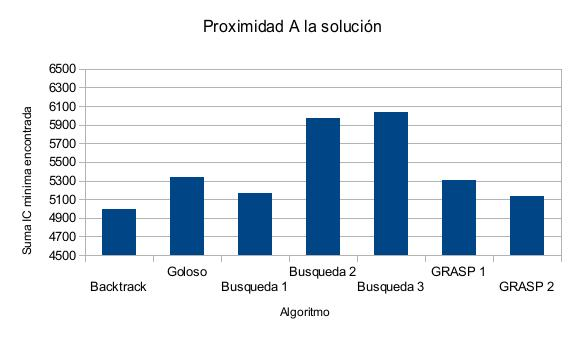
\includegraphics[scale=0.5]{Con/result.jpg}

Nuevamente puede observarse que las mejores heuristicas son las de busqueda local 1 y GRASP 2.

Y los tiempos obtenidos son:

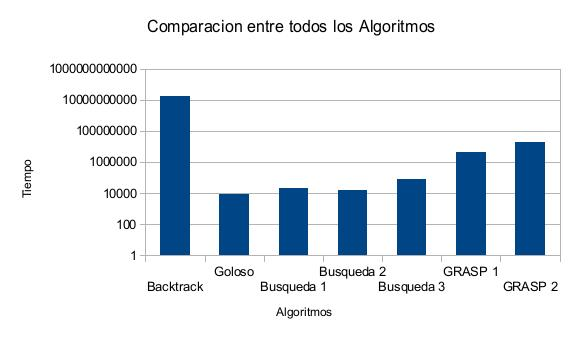
\includegraphics[scale=0.5]{Con/tiempos.jpg}

=========DECIR ALGO==============

\section{Conclución}


\clearpage

\section{Aclaraciones}
\section{Medicion de los tiempos}

Para este tp como trabajamos bajo el lenguaje de programacion C++, decidimos calcular los tiempos utilizando 'chrono' de la libreria standard de c++ (chrono.h) que nos permite calcular el tiempo al principio del algoritmo y al final, y devolver la resta en la unidad de tiempo que deseamos.\\ \\


\section{C\'odigo Fuente}
\subsection{Ej1.cpp}
\lstinputlisting[language=C++]{Ej1/ej1.cpp}

\newpage
\subsection{Ej2.cpp}
\lstinputlisting[language=C++]{Ej2/ej2.cpp}

\newpage
\subsection{Ej3.cpp}
\lstinputlisting[language=C++]{Ej3/ej3.cpp}



\end{document}